\documentclass[12pt]{article}
\title{ECE 11L Lab Report 1}

\author{Lawrence Liu}
\usepackage{graphicx}
\usepackage{amsmath}
\usepackage{subcaption}
\usepackage{array}

\begin{document}
\begin{titlepage}
   \begin{center}
       \vspace*{1cm}

       \textbf{EE 11L: Circuits Laboratory I}

       \vspace{2cm}

       \textbf{Experiment \#1}\\
       \textbf{Analog Discovery and Kirchhoff’s Laws}

            
       \vspace{4cm}
     
            
       Name: Lawrence Liu\\
		UID: 405749034\\
		Due Date: Nov. 11, 2100
            
   \end{center}
\end{titlepage}
\section*{Objectives}
To become familiar with basic circuit construction and operation of the Analog  Discovery 2 (AD2) device. Specially how to measure voltage, and resistance with the voltmeter and the impedance analyzer on the AD2. And to experimentally verify equivalent resistance and Kirchhoff’s Laws.
\section*{Theory}
Ohms Law
$$IR=V$$
Kirchhoff’s Voltage Law (sum of a loop of voltages is 0)
$$\sum V_i=0$$
Kirchhoff’s Current Law (sum of a node's currents is 0)
$$\sum I_k=0$$
\pagebreak
\section*{Experiment Setup: Lab 1}
\begin{figure}[h]
\includegraphics[width=8cm]{ResistorMeasurment}
\centering
\end{figure}
\section*{Measurements}
\begin{center}
\begin{tabular}{||c|c|c ||}
\hline
Resistance ($\Omega$) & Voltage (V) & Current (A)\\
\hline
\hline
$100\Omega$ & &\\
\hline
$680\Omega$ & &\\
\hline
$1200\Omega$ & &\\
\hline
\end{tabular}
\end{center}

\pagebreak
\section*{Discussion}
The Measured resistances were $100.1\Omega$, $704.3\Omega$, and $1194\Omega$ for the $100\Omega$, $680\Omega$, and $1200\Omega$ resistors. This falls within the given 5\% variance for each resistor.

Yes these values

The AD2 unit could measure the current and the resistance of the resistor by measuring the voltage drop across the reference resistor. Since this resistor's resistance is know, therefore, from ohms law the current across it can be calculated. Since the resistor being measured is in series with this one, that amount of current would also have to flow through that resistor. And since the voltage drop across this resistor and the current flowing across is know, its resistance can thus be derived. 
\pagebreak
\section*{Experiment Setup: Lab 2}
\begin{figure}[h]
\centering
\begin{subfigure}{.5\textwidth}
  \centering
  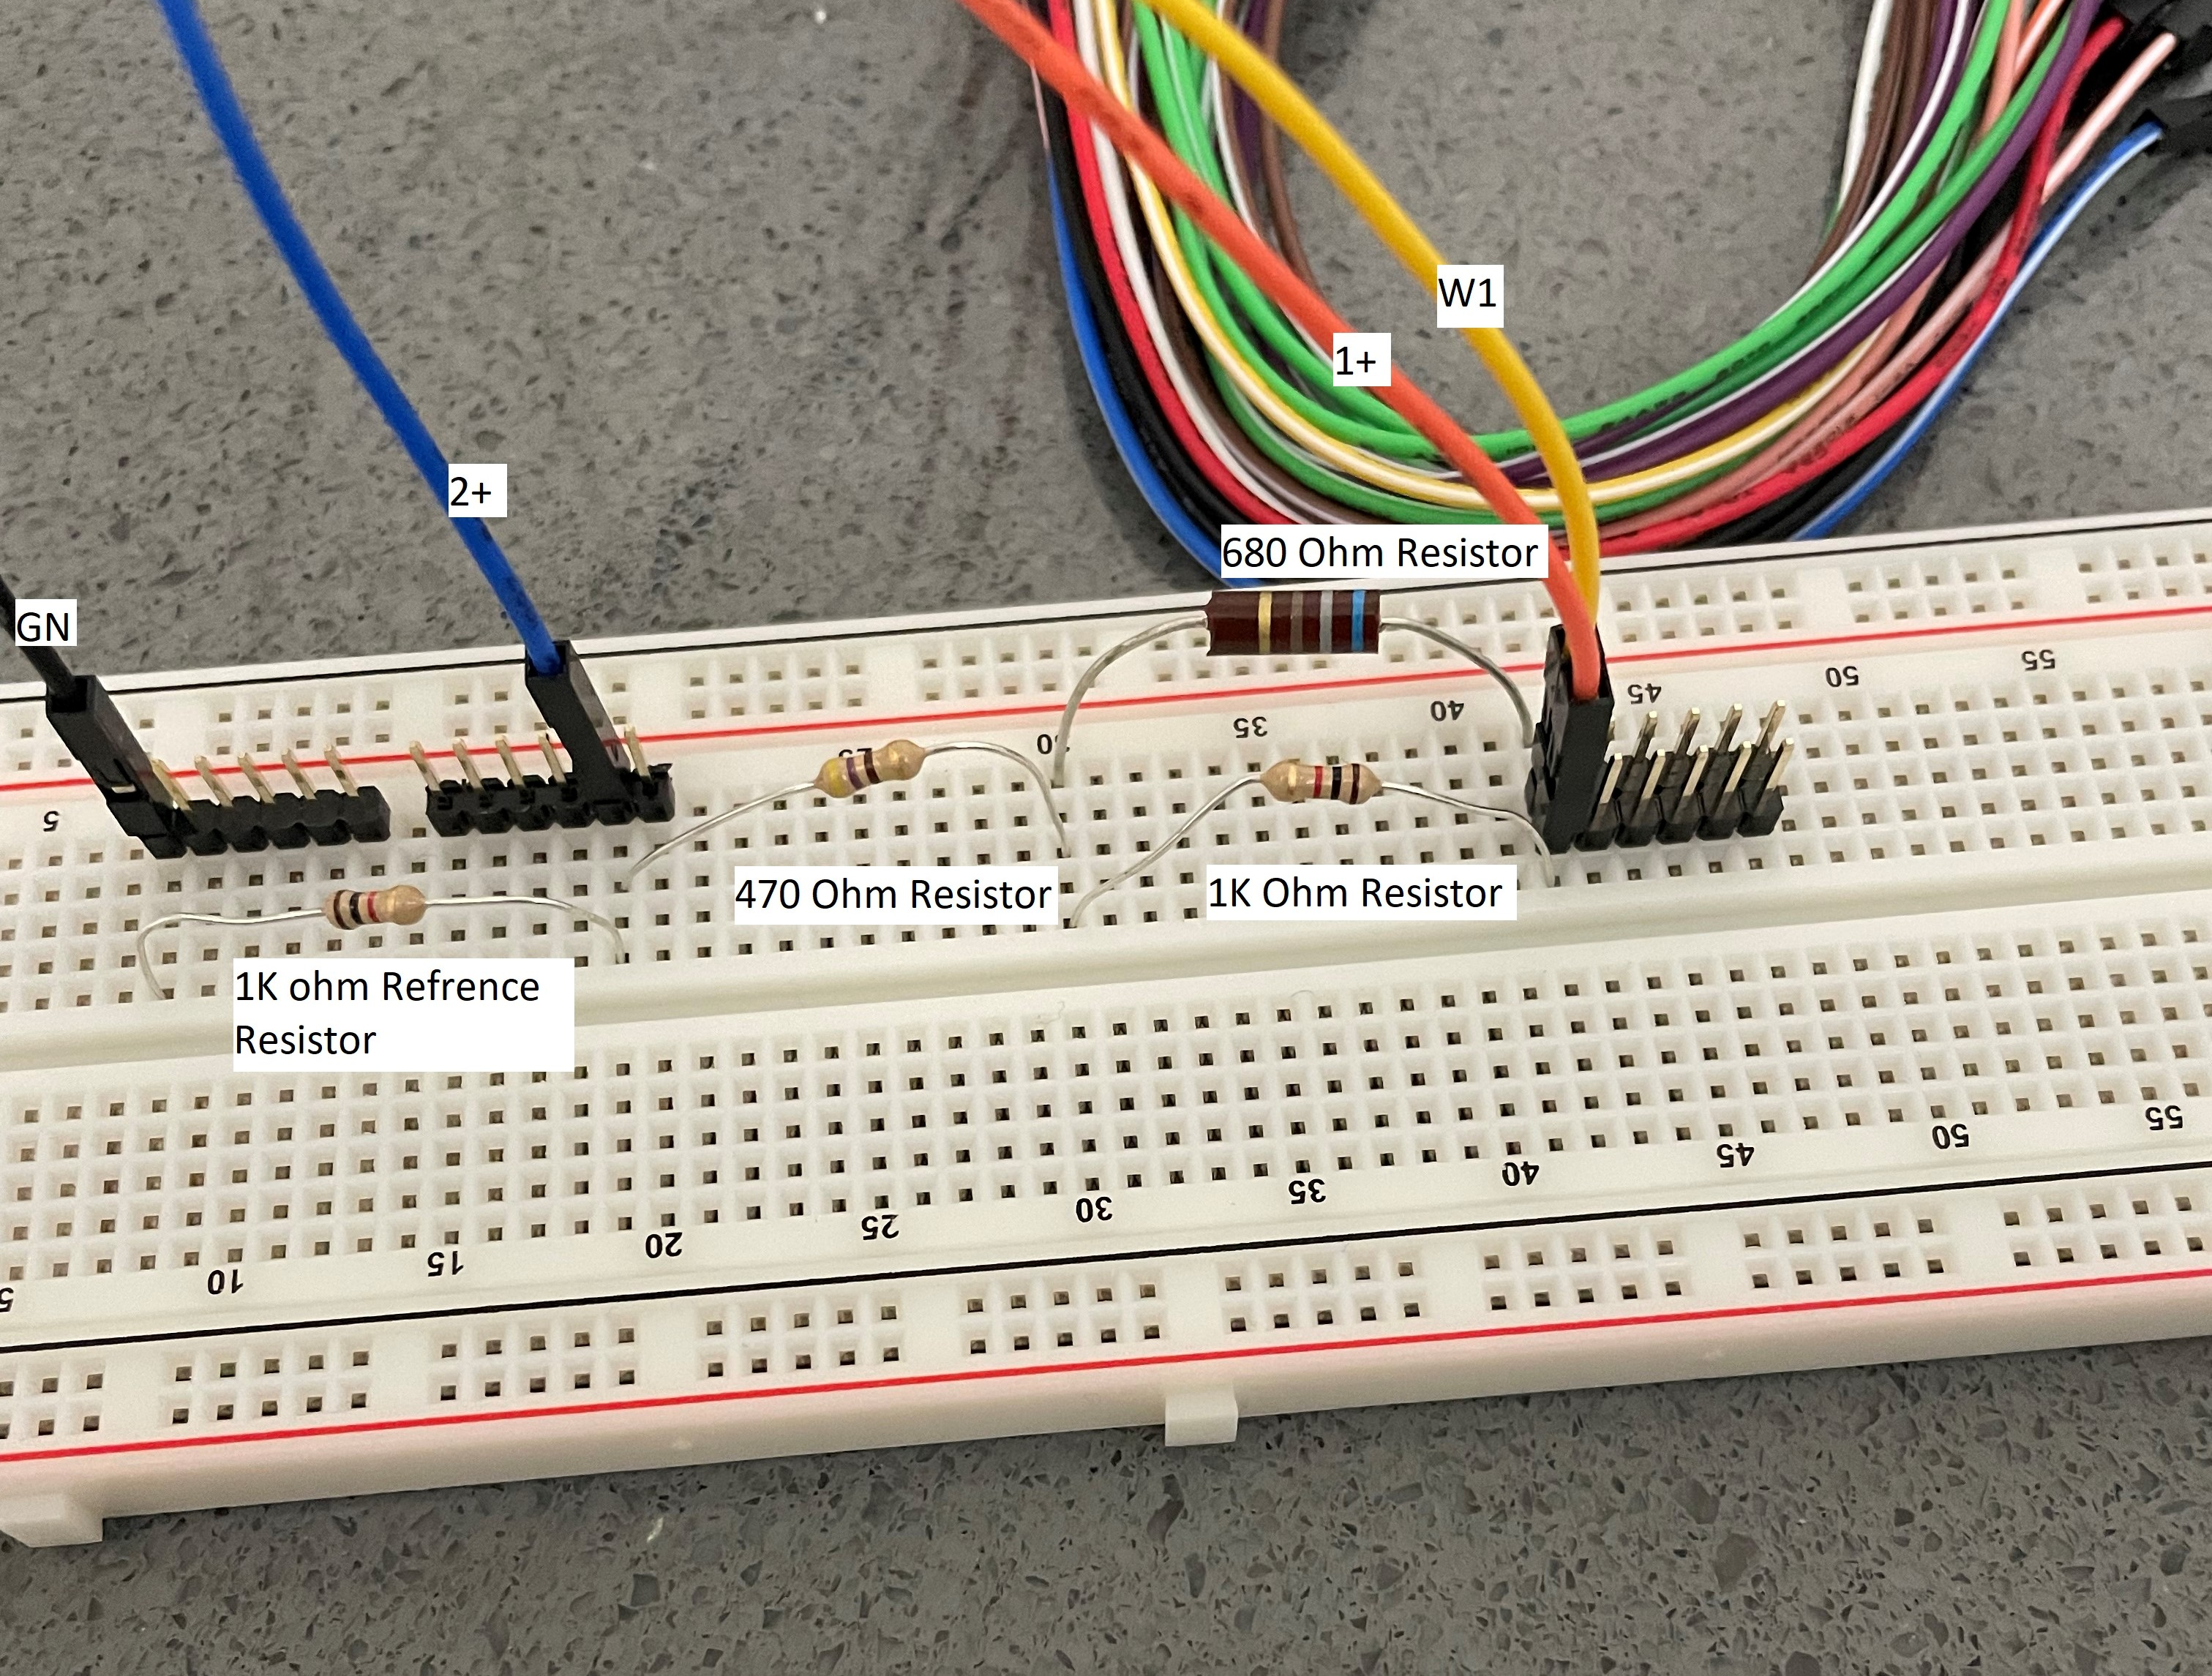
\includegraphics[width=.9\linewidth]{EquivalentResistance}
  \caption{The simple resistive network}
\end{subfigure}%
\begin{subfigure}{.5\textwidth}
  \centering
  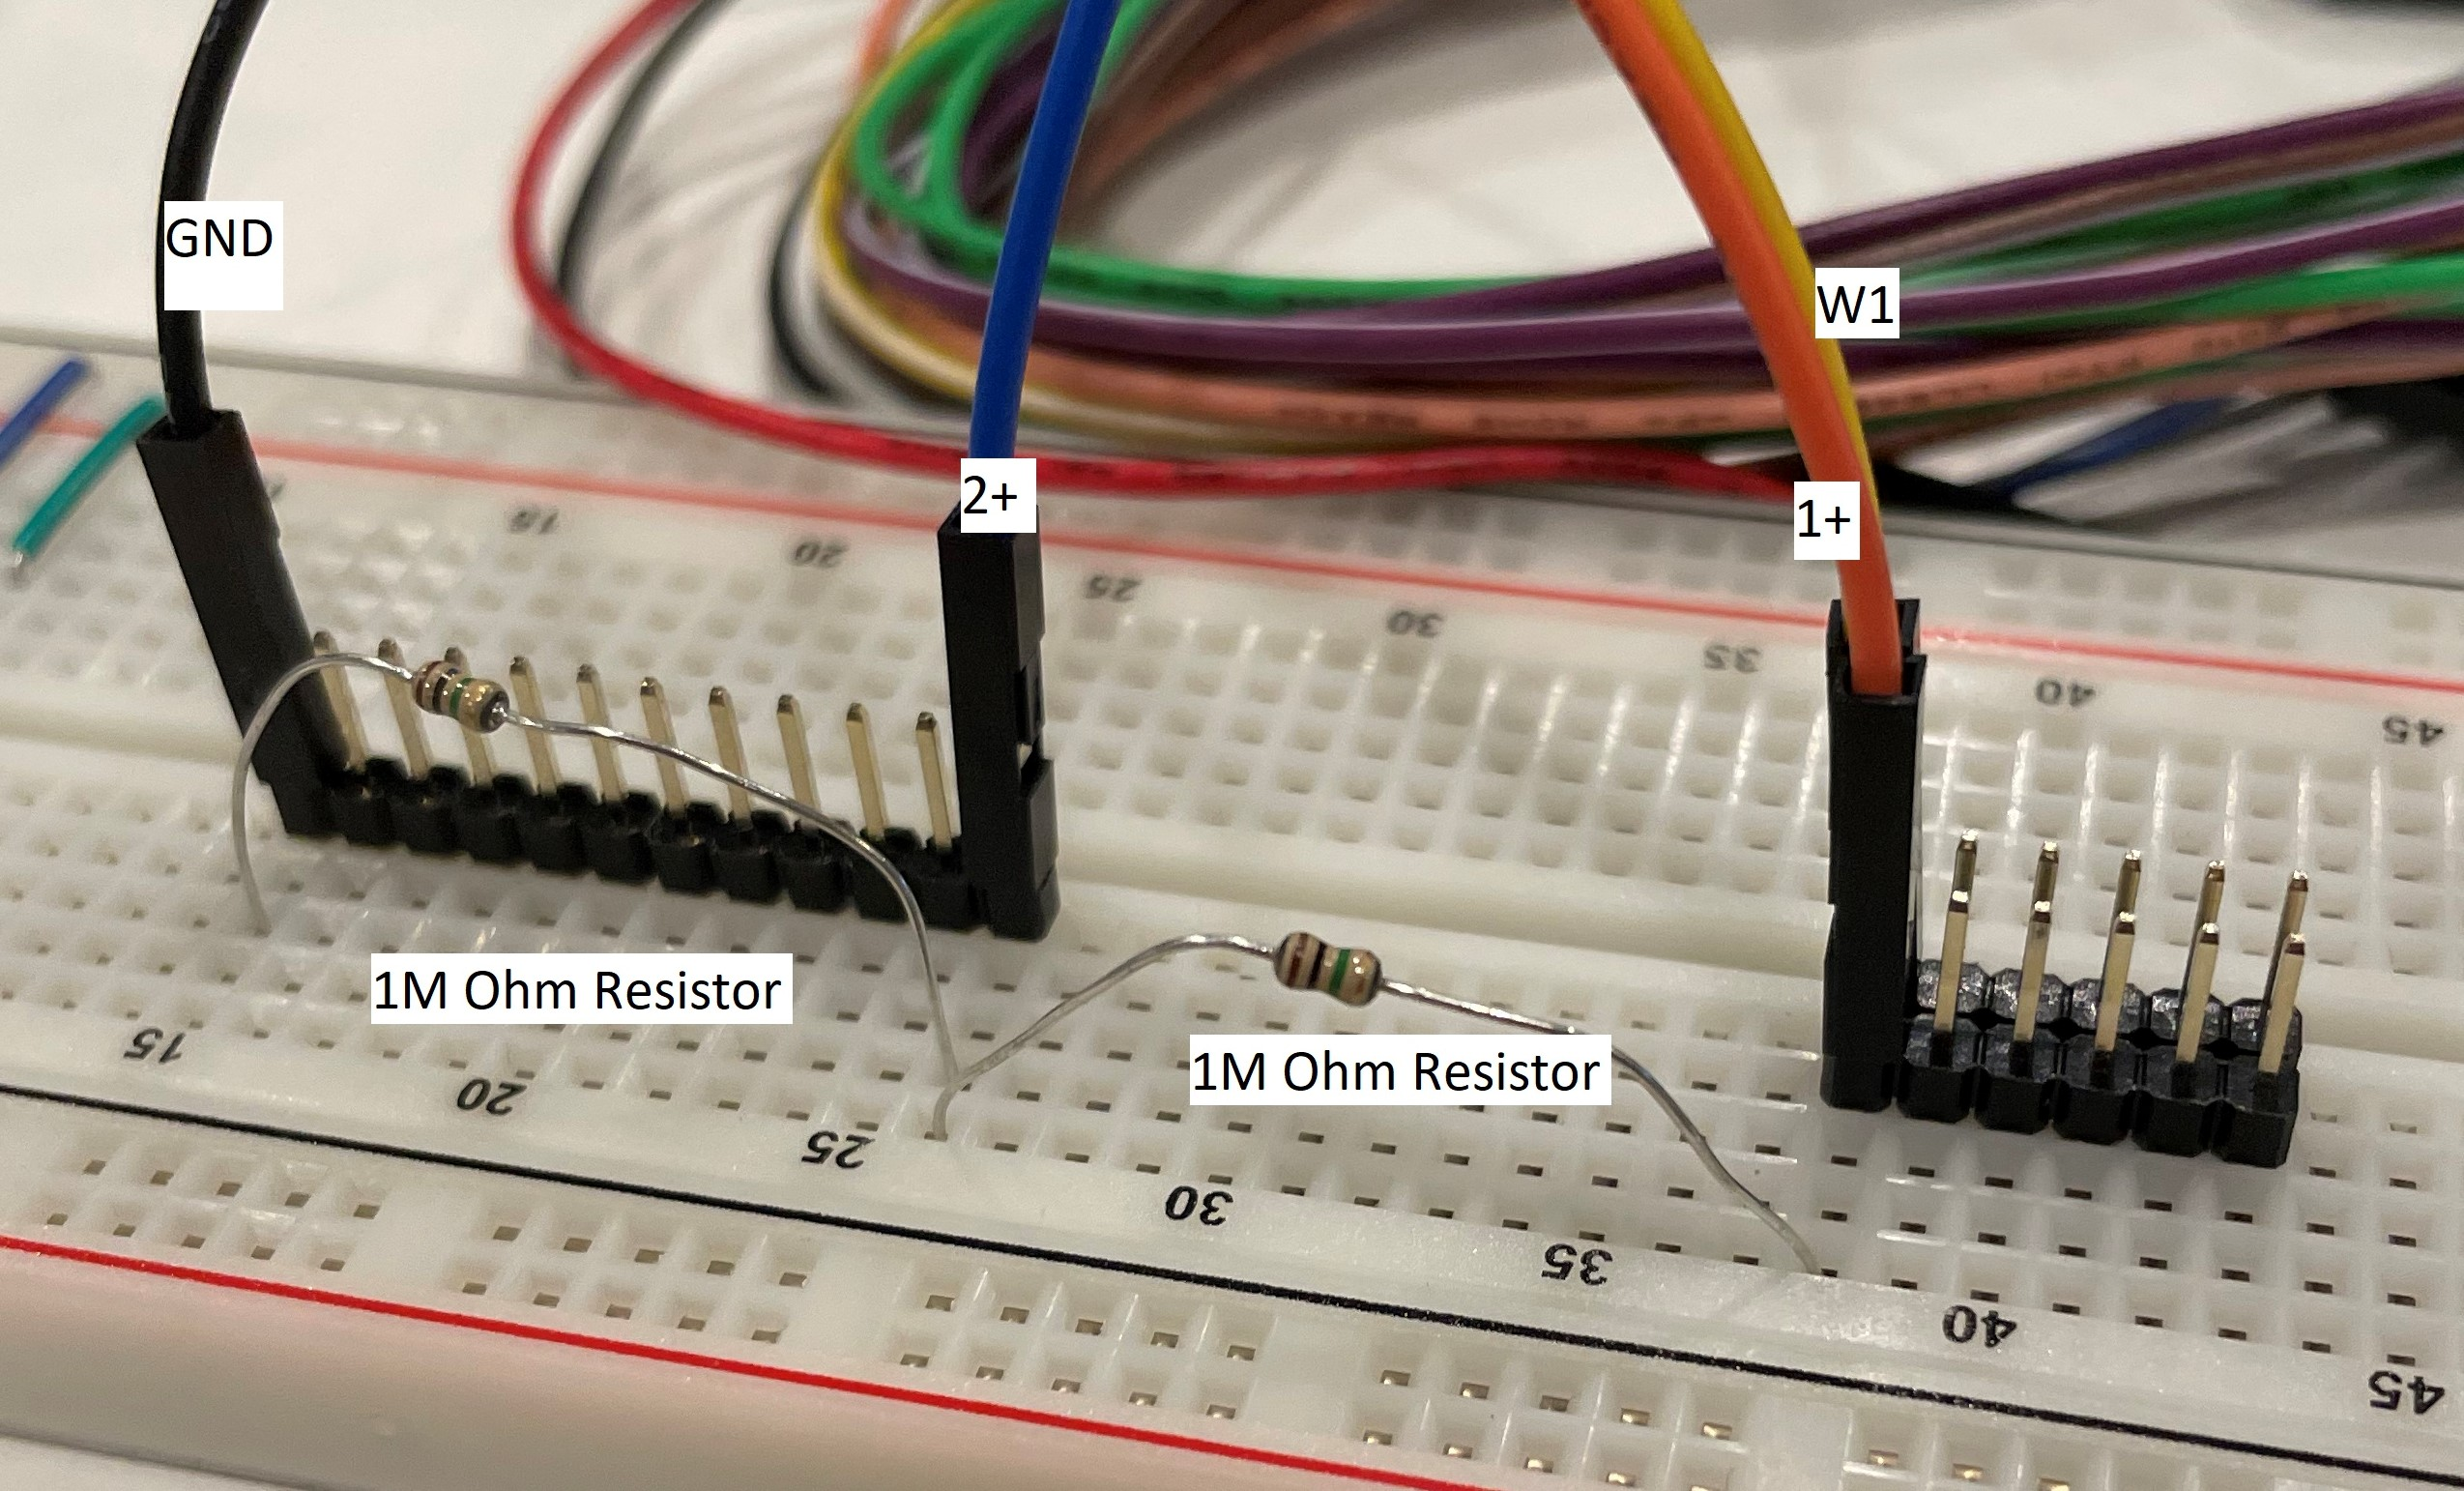
\includegraphics[width=.9\linewidth]{SkinResistor}
  \caption{The skin resistor setup}
\end{subfigure}
\end{figure}
The theoretical equivalent resistance for the simple resistive network is:
$$R_3+\frac{R_1R_2}{R_1+R_2}=874.76\Omega$$
The measured resistance is $876.6\Omega$, which agrees with the theoretical resistance given the 5\% variance of each resistor.

For the skin resistance experiment, I used a $1M\Omega$ resistor, when measured by the AD2, this resistor had resistance of $R_R=876.6k\Omega$. When measured in parallel with my "Skin Resistance", it was $R_{eq}=125.5k\Omega$. Thus my "skin resistance" was
$$R_{skin}=\frac{R_RR_{eq}}{R_R+R_{eq}}=109.78K\Omega$$
\pagebreak
\section*{Discussion: Lab 2}
Since my skin resistance is $109.78K\Omega$, from ohms law at $50V$, $0.00045A$ would flow through my body.
\pagebreak
\section*{Experiment Setup: Lab 3}
\begin{figure}[h]
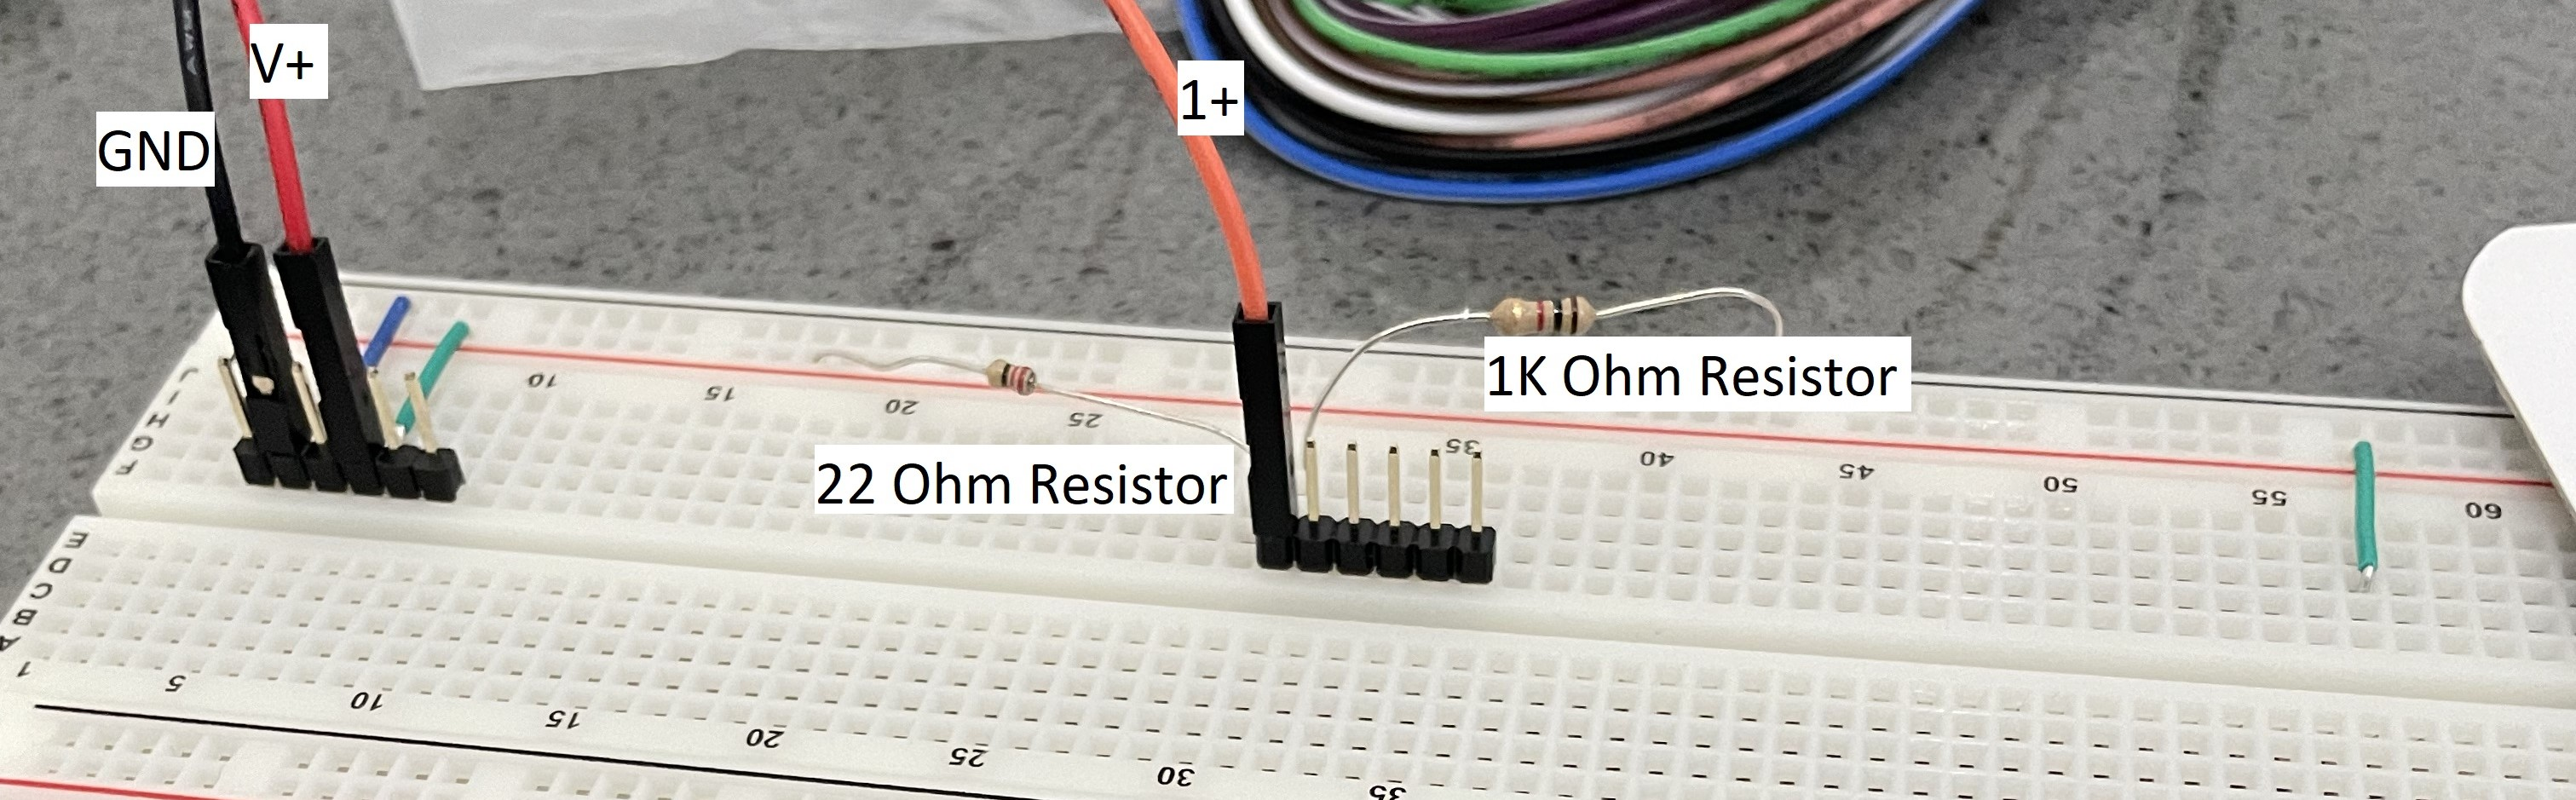
\includegraphics[width=8cm]{VoltageDivider}
\centering
\caption{Voltage Divider}
\centering
\end{figure}
\begin{figure}[h]
\includegraphics[width=8cm]{CurrentDivider}
\centering
\caption{Current Divider}
\centering
\end{figure}
\begin{figure}[h]
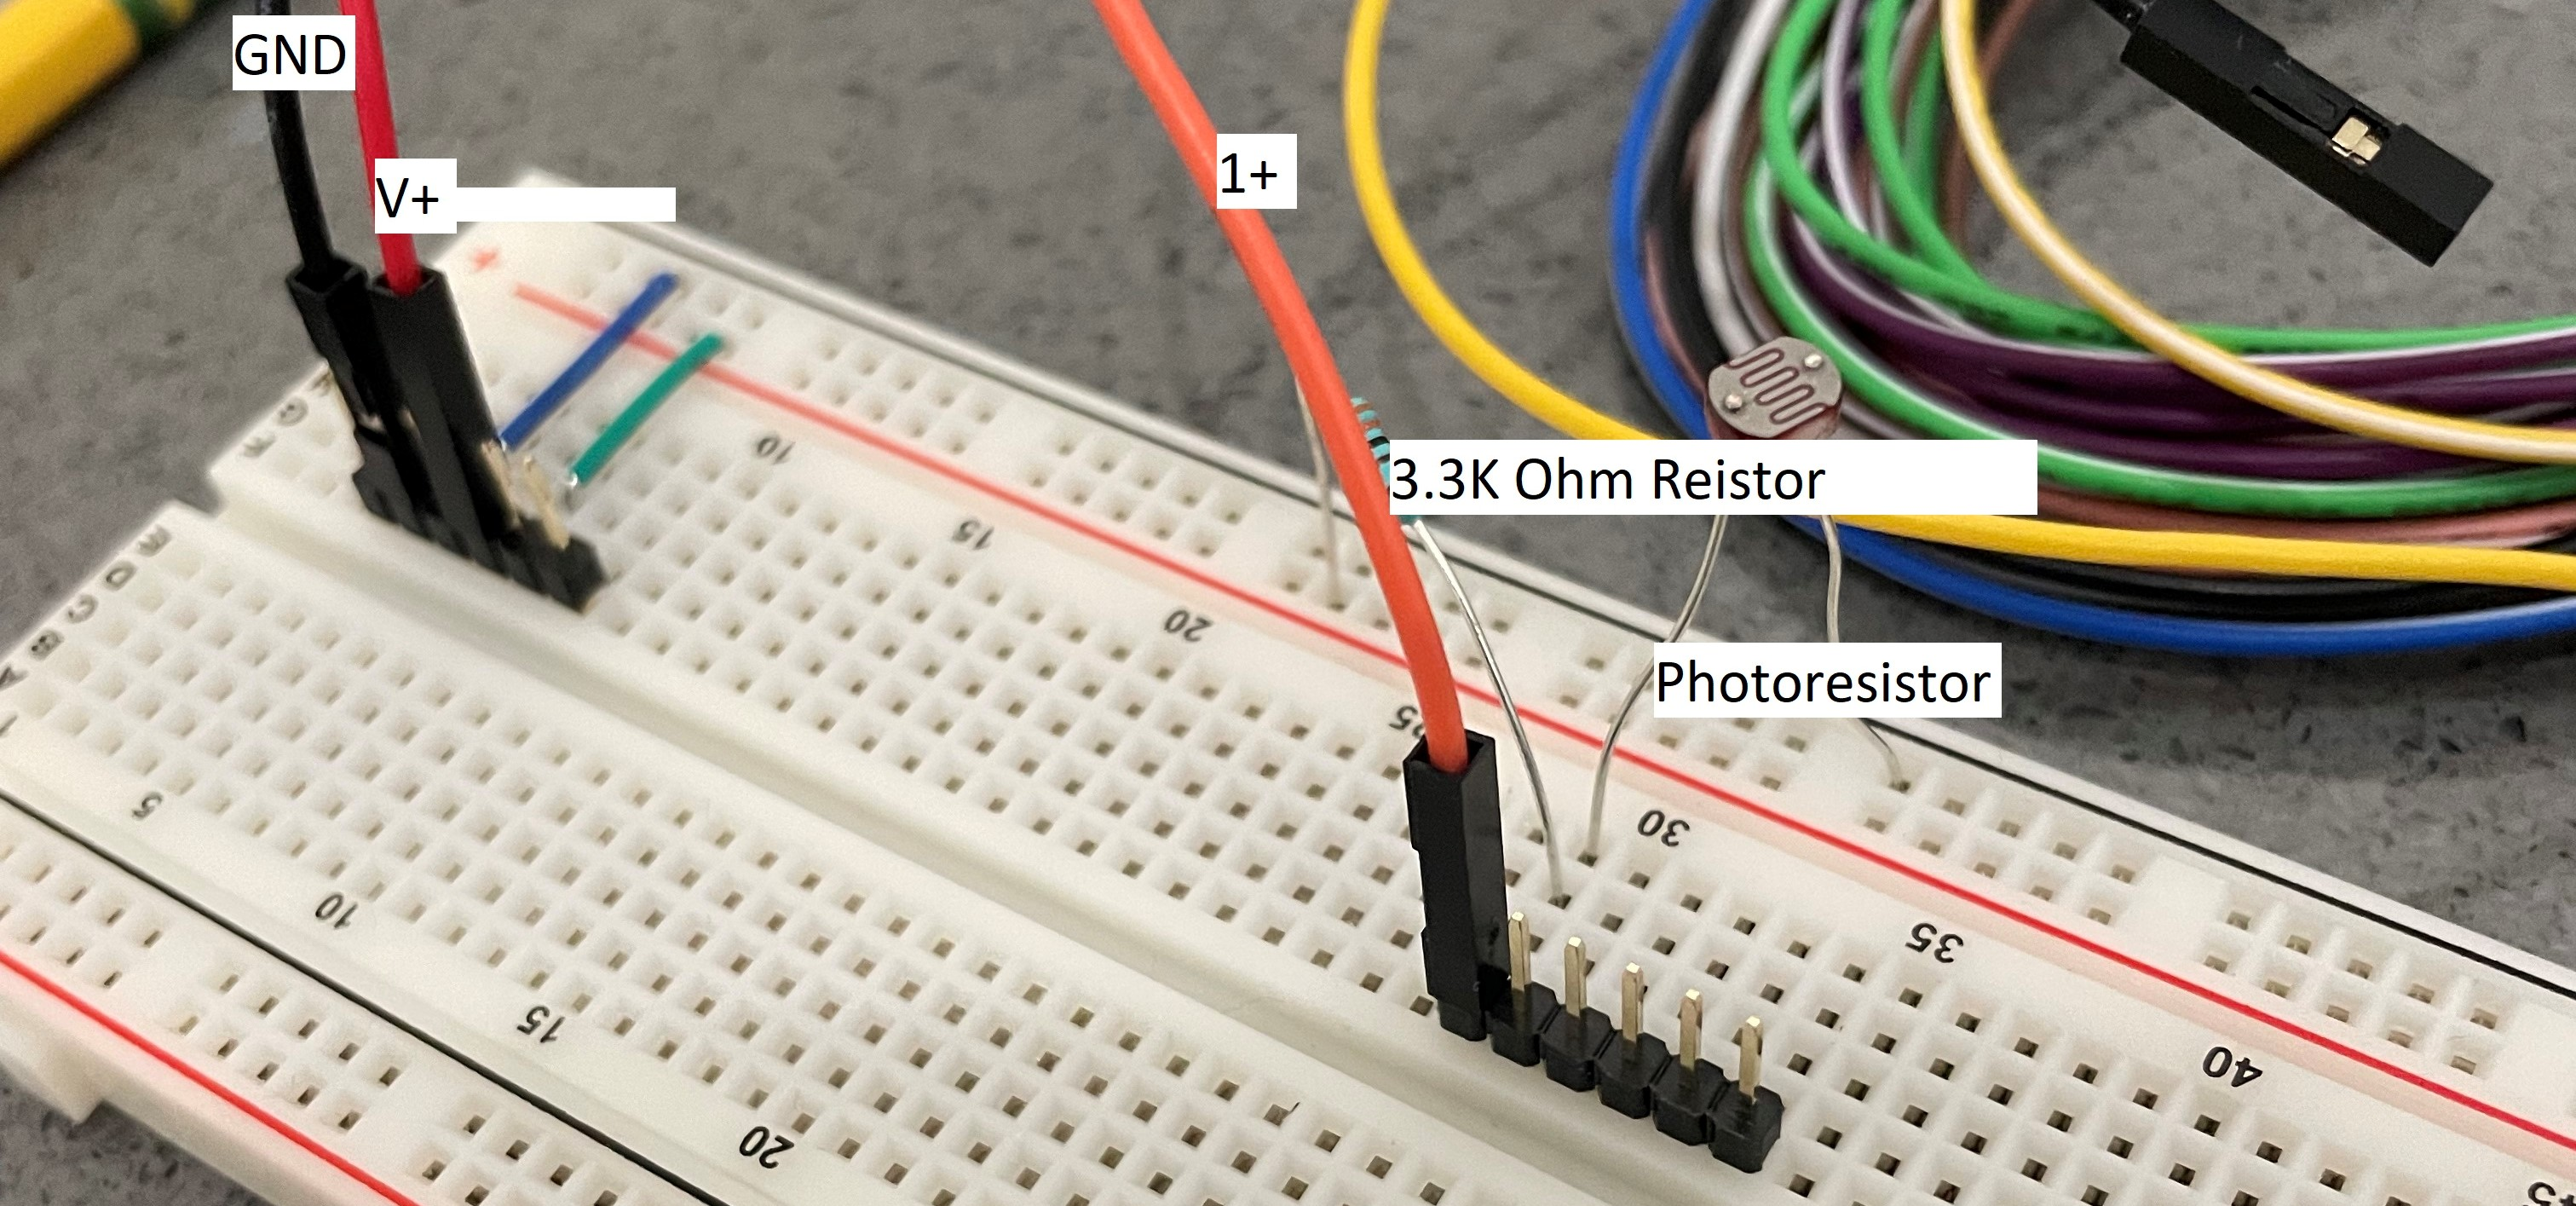
\includegraphics[width=8cm]{PhotoResistor}
\centering
\caption{Photoresistor}
\centering
\end{figure}
\section*{Data}
\subsection*{Voltage Divider}
\begin{center}
\begin{tabular}{||c|c|c ||}
\hline
Resistors ($\Omega$) & Theoretical Voltage (V) & Measured Voltage (V)\\
\hline
\hline
$22\Omega$  &0.108V &0.104V\\
\hline
$1000\Omega$ &4.892V &4.896V\\
\hline
\end{tabular}
\end{center}
\subsection*{Current Divider}
\begin{center}
\begin{tabular}{||m{1.5cm}|m{2cm}|m{2cm}|m{2cm}|m{2cm}||}
\hline
Resistors ($\Omega$) & Theoretical Voltage (V) & Measured Voltage (V) & Theoretical Current (A) & Measured Current (A)\\
\hline
\hline
$22\Omega$ & 0.322V & 0.318V&0.014A &0.014A\\
\hline
$1000\Omega$ &4.678V &4.682V &0.004A &0.004A\\
\hline
$470\Omega$ &4.678V &4.682V &0.01A &0.01A\\
\hline
\end{tabular}
\end{center}
\subsection*{Photoresistor}
\begin{center}
\begin{tabular}{||c|c ||}
\hline
Lighting & Measured Voltage (V)\\
\hline
\hline
Standard Lighting & 2.562V\\
\hline
Dark Room  &4.874V\\
\hline
\end{tabular}
\end{center}
\section*{Discussion: Lab 3}
The theoretical and measured values for the voltages and currents were fairly close. For the Voltage dividers the difference between the measured voltages and the actual voltages were only $0.08\%$ and $3.7\%$ for the $1000\Omega$ and $22\Omega$ resistors respectively. For the current  Current divider the difference between the measured and theoretical current was $0\%$ for all resistors.

The photoresistor's resistance increased as the amount of light it was exposed to decreased. At standard lighting, its measured resistance was around $3.3K\Omega$, however when it was placed in a dark room, its resistance increased to around $130K\Omega$

\end{document}